\section{Sharing Descriptive Categories} % TODO: Find better name

With our case representations, we first look at cases used in different treebanks as representing the values of a descriptive category.
We want to know how relevant is to apply the same name to values of a similar category in different languages.
%is reusing the same names for cases in different languages.

First, we compare case labels from two closely related languages, namely Czech and Russian\footnote{We tried a number of pairs and decided to just present Czech and Russian for space reason.}.
To do so we compute the euclidean distance between each case in the first language and each case in the second language. 
Then, we generate a 1-nearest neighbour graph assuming the neighbours of a node must come from the other language. % where a node representing a case in the first language has an out edge to the nearest node representing a case in the other language.
This gives us an idea of the way cases could be mapped in a transfer learning setting for example.

\begin{figure*}
    \begin{center}
    \hfill
    \newdimen\height
    \setbox0=\hbox{%
    \begin{minipage}{.75\textwidth}
    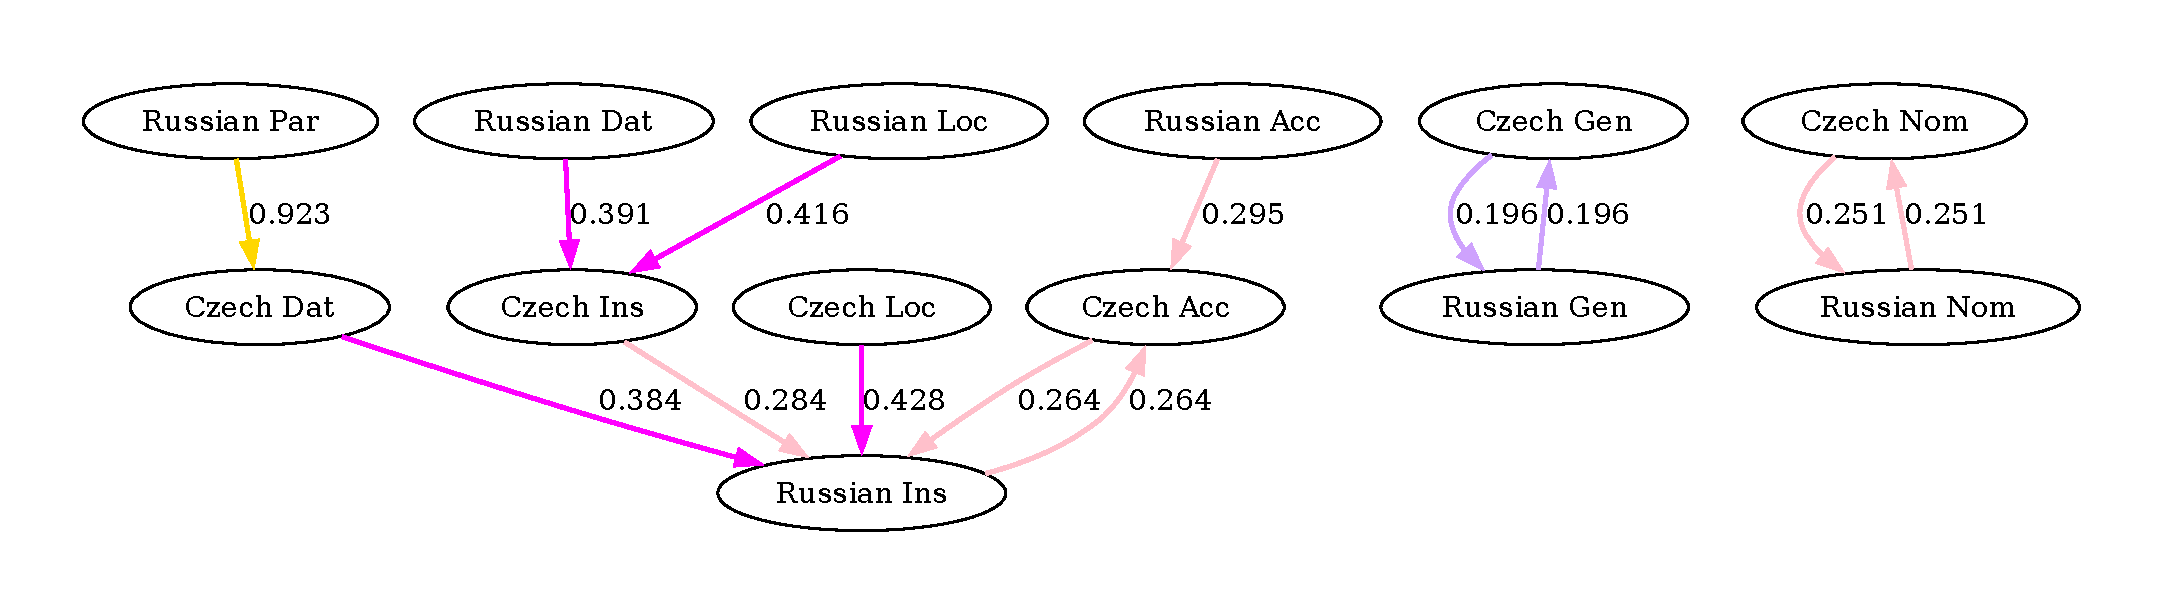
\includegraphics[width=\linewidth]{Images/gnn_Case_Only_cs_cltt-ud-dev_ru_gsd-ud-dev.pdf}
    \captionof{figure}{Graph of Nearest Neighbours for Czech CLTT and Russian GSD}
    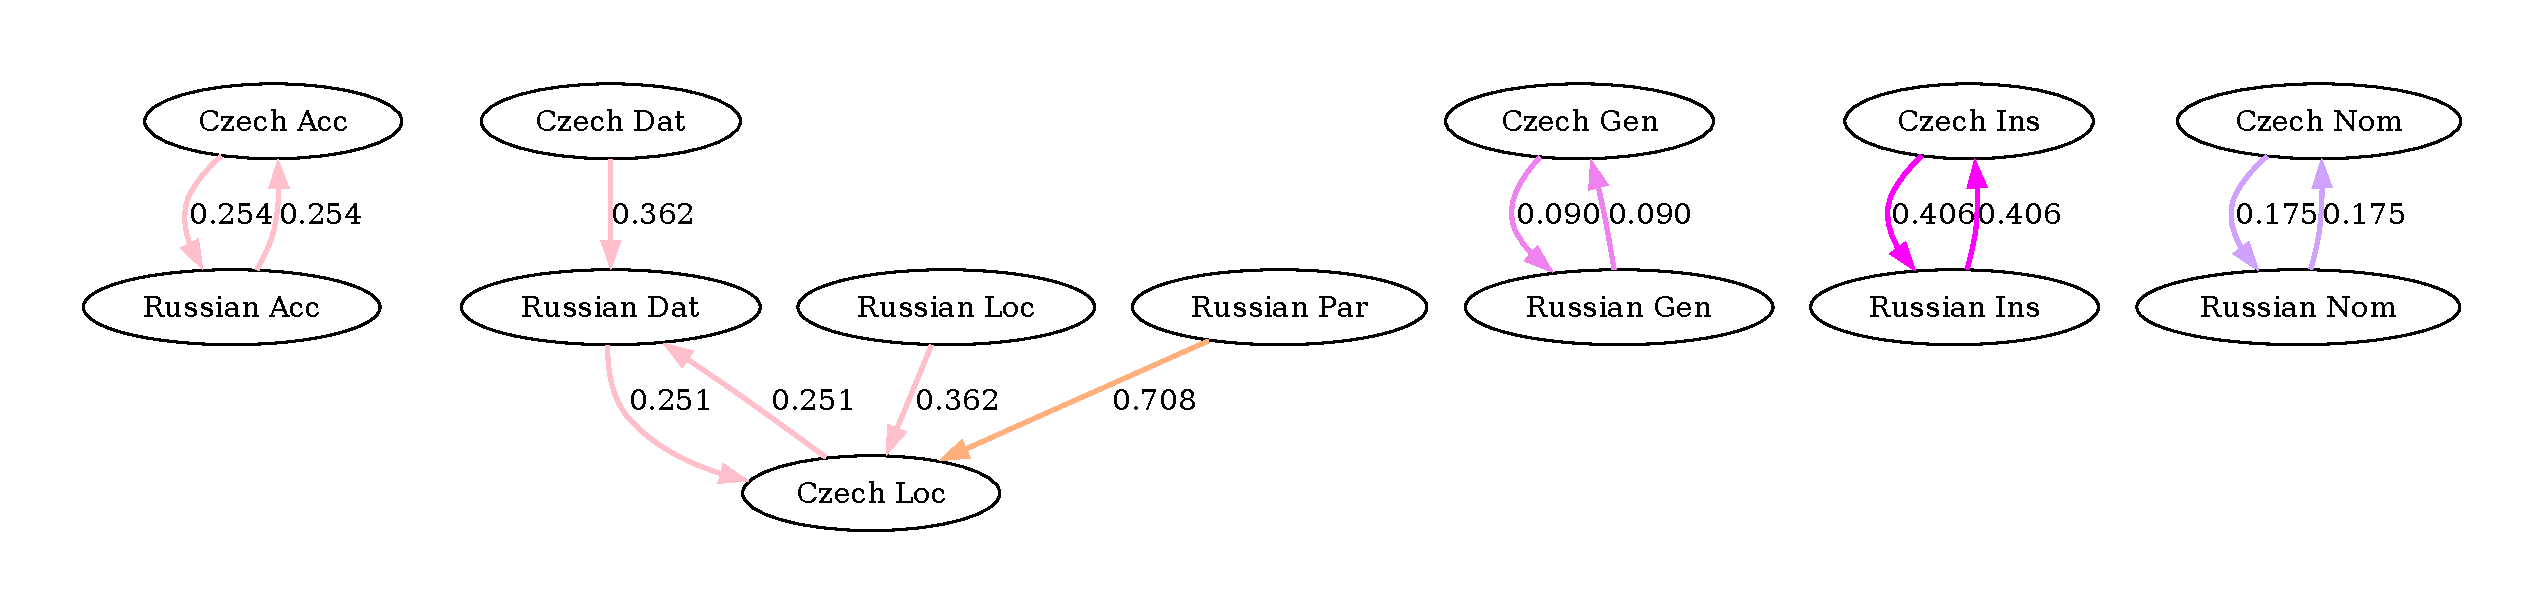
\includegraphics[width=\linewidth]{Images/gnn_Nouns_Case_Only_cs_cltt-ud-dev_ru_gsd-ud-dev.pdf}
    \captionof{figure}{Graph of Nearest Neighbours for Nouns in Czech CLTT and Russian GSD}
    \end{minipage}}
    \height=\ht0 \advance\height by \dp0
    \addtocounter{figure}{-2}
    
    \begin{minipage}{.8\textwidth}
    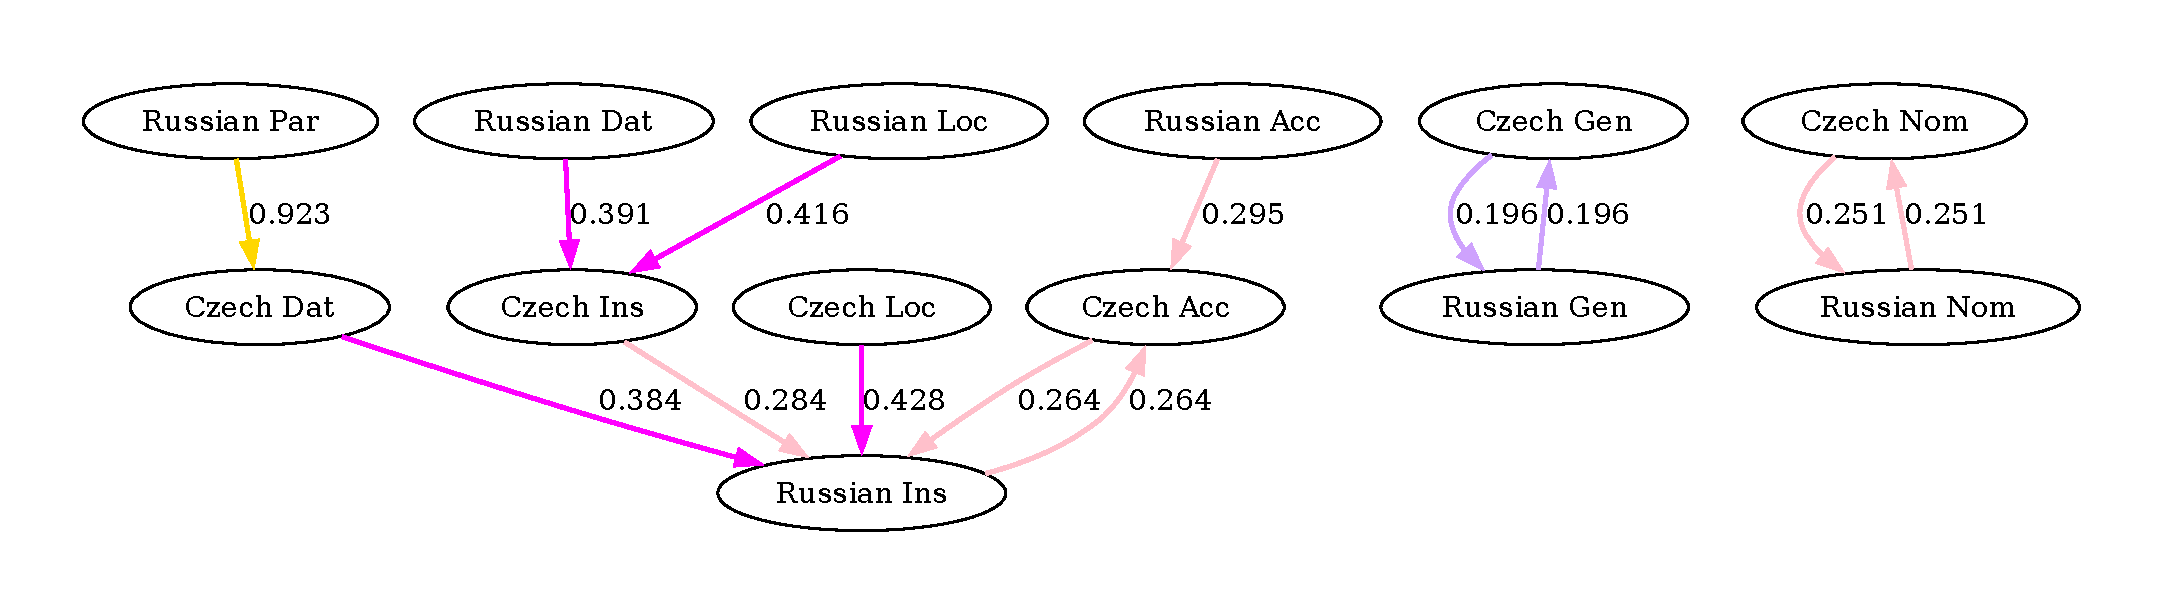
\includegraphics[width=\linewidth]{Images/gnn_Case_Only_cs_cltt-ud-dev_ru_gsd-ud-dev.pdf}
    \captionof{figure}{Nearest neighbour graph for Czech CLTT and Russian GSD case profiles. 
    The corresponding distance matrices are tables 5, 7 and 9 in the appendix.}
    \label{fig:allpos}
    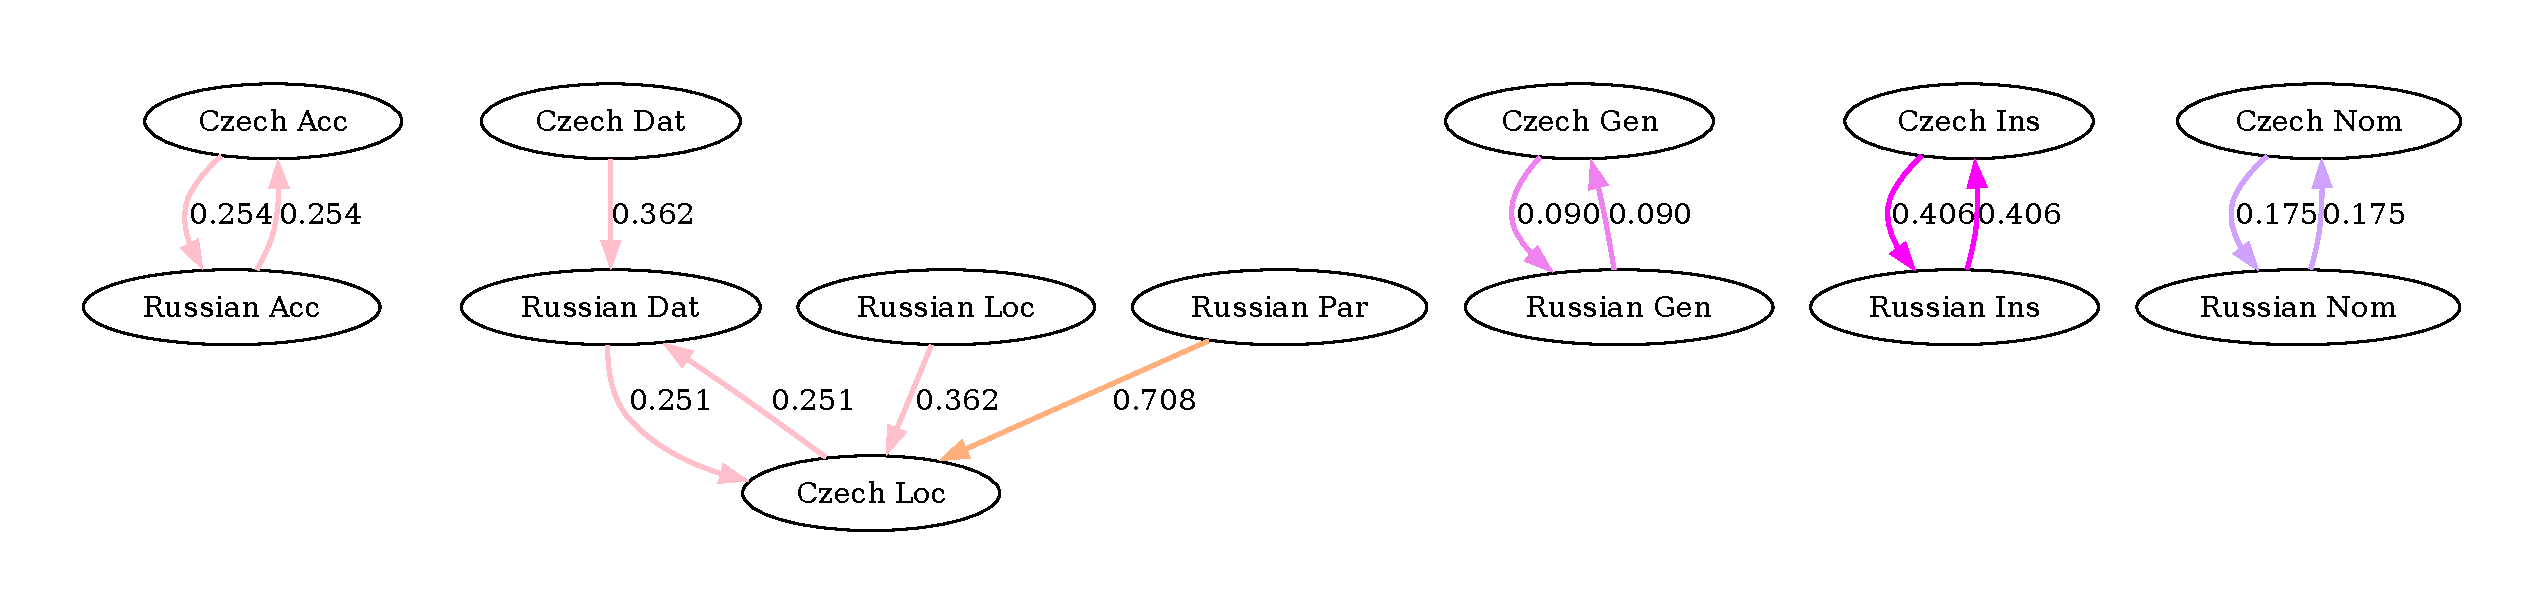
\includegraphics[width=\linewidth]{Images/gnn_Nouns_Case_Only_cs_cltt-ud-dev_ru_gsd-ud-dev.pdf}
    \captionof{figure}{Nearest neighbour graph Czech CLTT and Russian GSD case profiles of nouns.
    The corresponding distance matrices are tables 6, 8 and 10 in the appendix.}
    \label{fig:noun}
    \end{minipage}
    \hfill
    \begin{minipage}{.15\textwidth}
    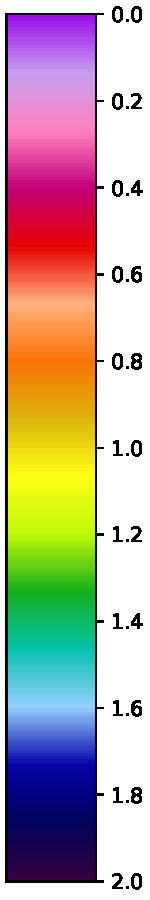
\includegraphics[height=\height]{Images/bar.pdf}
    \end{minipage}
    \hfill
    \end{center}
    \label{fig:gnn_ru_cs}
\end{figure*}

%To avoid the repetition and overabundance of some dependency relations (such as \texttt{case, det, amod}\ldots), we also printed the same graph when only taking into account nouns. 
%This allows for our embedding of cases to be a better representation of the part a case plays in the sentence, as it is then not repeated for each word in a noun group. 
%In the same goal, we also avoid the \texttt{conj} dependency relation. 
%This comes from the fact a case applies to a whole noun group more than just a word, except for noun groups being parts of noun groups.
%\medskip

%!!!!! assuming a case category in russian and a value for it called dative...

Figure \ref{fig:allpos} represents the 1-nearest neighbour graph of Czech and Russian cases when representations are computed over all the words marked for case.
We see that the Czech and Russian \scsf{nominatives} are each other's nearest neighbour and such is the case for the two genitives.
However, for the other cases, the picture is less clear.
This is likely due to the fact that when we compute the representations using all the parts-of-speech at once, we confuse the different types of case assignment.

Figure \ref{fig:noun} which represents the 1-nearest neighbour graph of Czech and Russian cases when representations are computed only on nouns, is clearer.
On top of the \scsf{nominatives} and \scsf{genitives}, the \scsf{accusatives} and \scsf{instrumentals} are also each other's nearest neighbours.
Only the \scsf{datives}, \scsf{locatives} and Russian \scsf{partitive} are still entangled.
Looking directly at the data, we realize that the \texttt{iobj} relation is never used in the Czech CLLT corpus.
The increased probability of seeing a noun in the \scsf{dative} descending from an \texttt{obl} relation makes the Czech \scsf{dative} more distinct from the Russian \scsf{dative} and the Czech \scsf{locative} is.

Note that not all pairs of languages are as well behaved as Czech and Russian, as we shall see in section 6.

%Notably, the graphs about every Part of Speech (PoS) and about Nouns only are very similar in structure. 
%When building more graphs comparing more languages and more paradigms, we see a similar pattern arise. 
%However, we have a huge volatility in graphs depending on the number of inputs. 

%On these graphs, we see for example that the Russian dative is closer to the Czech instrumental than it is of the Czech dative.


%For example, there are much fewer samples of pronouns with a certain case than samples of nouns with that same case, making the graph change a lot between considered corpora. 
%It appears that using pronouns only limits the quantity of information available to create graphs while using them in addition to nouns makes for redundant information. 